\newpage
\begin{appendices}
\iftoggle{toclinks}{\gototoc}{} % Turn it on/off in packages.tex, command in macros.tex
\iftoggle{cboxes}{	   				  % Turn it on/off in packages.tex
	\begin{boxeditems}
		\item Add link to website for Excel file with tickers.
		\item Add reference to paper that compares YC from Bloomberg for the Euro area.
	\end{boxeditems}}{}


\section{Trend Inflation as a Proxy for Long-Term Inflation Forecasts} \label{sec:trendinf}

An advantage of the small open economy approach is that it only requires forecasts for inflation, or a proxy in the case of countries with no long-term forecasts available as is the case for Israel and South Africa.
Inflation expectations are hoped to match measures of inflation that exclude unexpected shocks and better reflect the inflation environment.
Different measures of core inflation exist.
I use the inflation trend obtained by applying the Hodrick-Prescott filter to the series of realized inflation of each country.
Of course, the filter is sensitive to the sample period used.
The resulting trend can also be outside of the target inflation band due to the innate dynamics of the series, which would be at odds with survey data (see figure \ref{fig:wnCPI}).
Fortunately, unlike other countries, there is no marked upward or downward trend in the inflation of the two countries during the sample period.
For each country, trend inflation is calculated for the whole period but only considered within the time range for which survey data is available for the rest of the countries, and as long as the trend is within the inflation target band.
Figure \ref{fig:CPI_ILSZAR} shows the realized and trend inflation for Israel and South Africa, and compares them with those of Malaysia and Thailand, two countries with a similar pattern for inflation (i.e. no marked trend) and for which survey data is available.
%It supports that t
Trend inflation seems to be a good proxy for the long-term inflation forecasts of Israel and South Africa.
Finally, since the 5-year and long-term forecasts closely follow each other (see figure \ref{fig:wnCPI}), I use trend inflation for both tenors.

\begin{landscape}
	\documentclass{article}
\usepackage{graphicx}
\usepackage[margin=1in]{geometry}
\usepackage[outdir=./]{epstopdf}  					% Avoids errors when input figures
\usepackage[labelsep=period,labelfont=bf]{caption}
%\usepackage{subcaption}

\begin{document}

\begin{figure}[tbph]
	\begin{center}
		\caption{Trend versus Long-Horizon Forecasts of Inflation}
		\label{fig:CPI_ILSZAR}
		\includegraphics[trim={0cm 0cm 0cm 0cm},clip,height=1\textheight,width=1.4\textwidth]{../Figures/Surveys/CPI_ILSZAR.eps} \\
	\end{center}
	% trim = {<left> <lower> <right> <upper>}
%	\vspace{-0.4cm} \caption*{\footnotesize{\textit{Notes}: Notes.}}
\end{figure}

\end{document}
\end{landscape}

%		\begin{figure}[!htbp]
		\begin{centering}
			\vspace{12.5mm}
			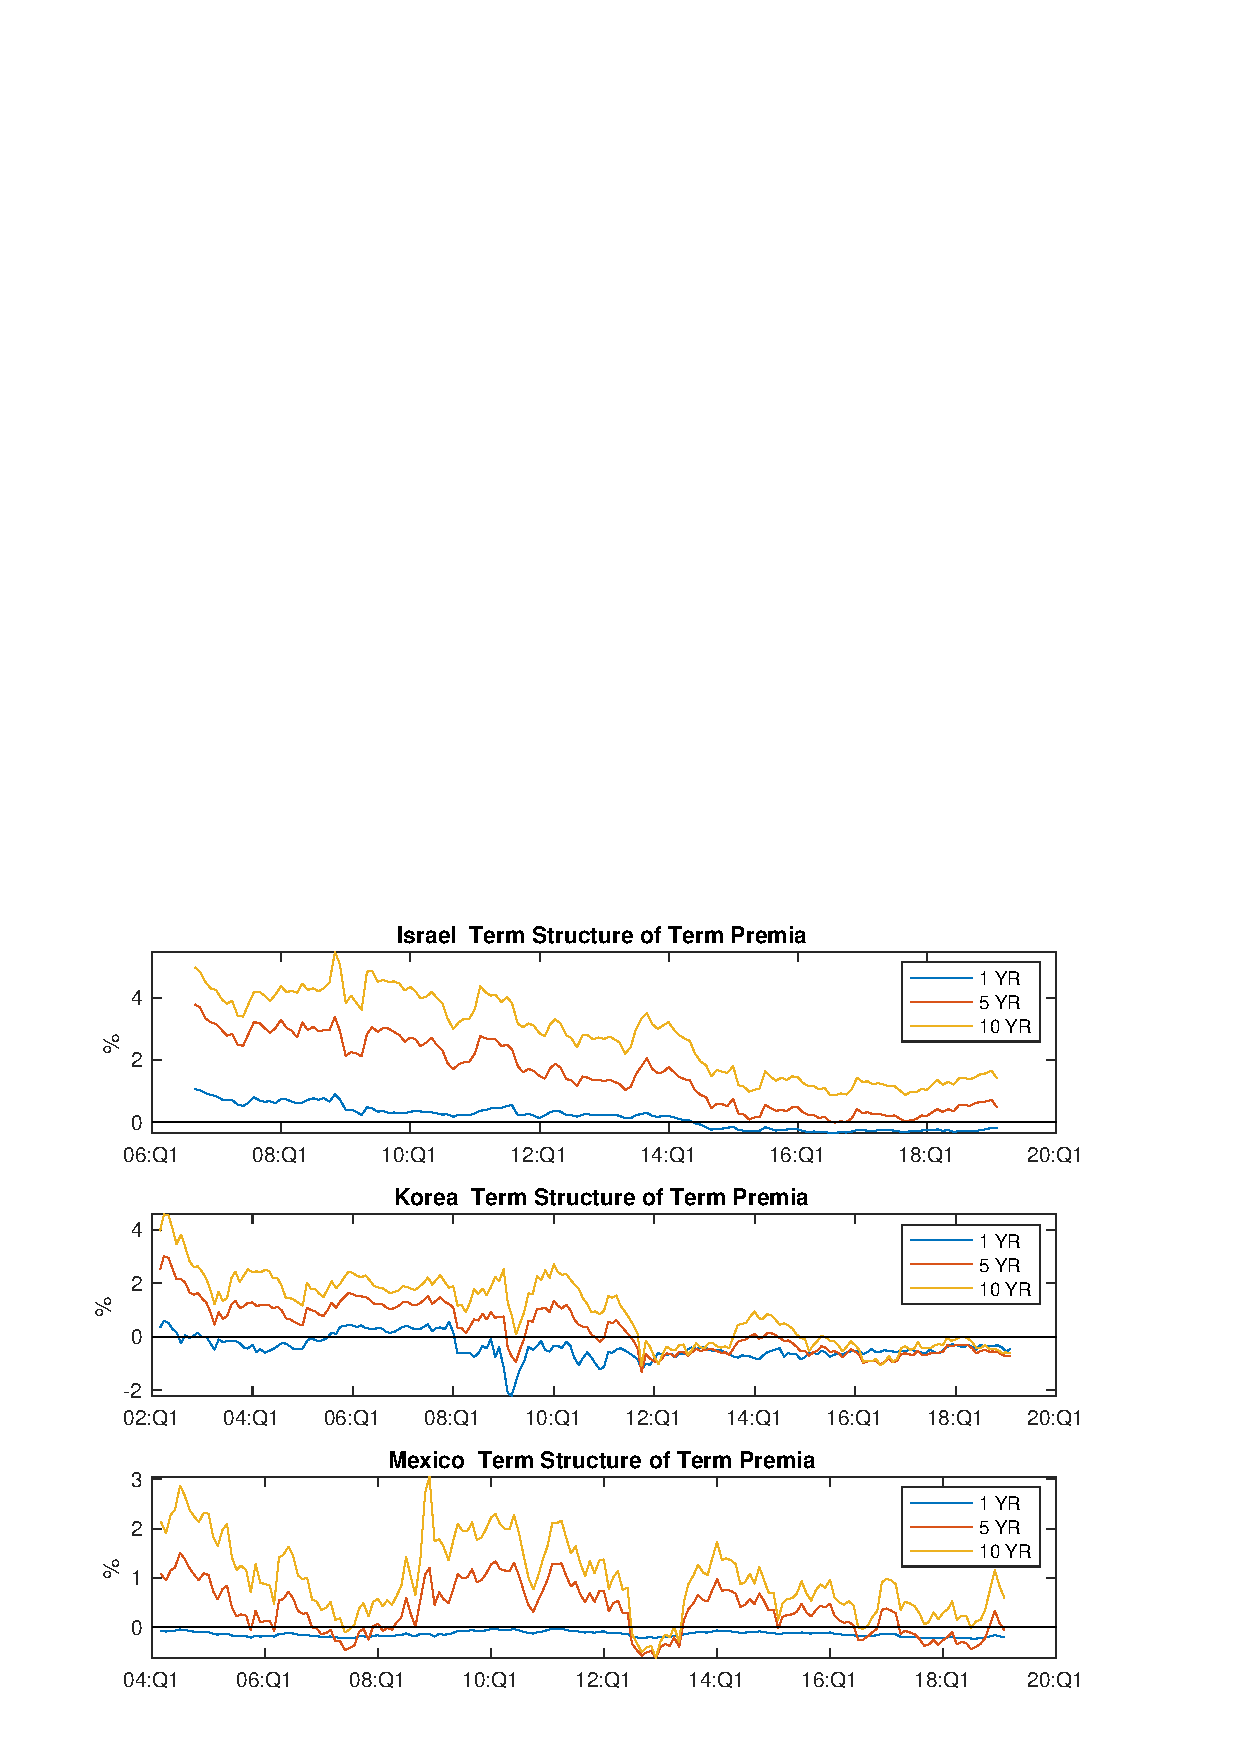
\includegraphics[width=1\textwidth,height=0.8\textheight]{../Figures/Temp/temp_ts_tp}
			\par\end{centering}
		\caption{Estimated Term Premia for Different Maturities.}\label{fig:temp_ts_tp}
	\end{figure}

%\newgeometry{top=4cm, left=5.5cm}	% Modify this if more space is needed
%%\newgeometry{margin=1cm}  % To make the table fit your landscape
%\begin{landscape}
%	\begin{table}
\centering
\begin{tabular}{l|cccccccccccccc}
\toprule
&\textbf{COP}&\textbf{HUF}&\textbf{IDR}&\textbf{ILS}&\textbf{MXN}&\textbf{PEN}&\textbf{PHP}&\textbf{PLN}&\textbf{TRY}&\textbf{KRW}&\textbf{MYR}&\textbf{RUB}&\textbf{THB}&\textbf{ZAR}\\\midrule
{ Coeff.}&1.17&-0.28&-0.32&1.02&0.42&1.50&-0.14&0.43&1.41&1.02&-0.23&1.37&0.82&-0.35\\\
{S.E.}&0.24&0.15&0.20&0.11&0.15&0.32&0.24&0.11&0.27&0.12&0.10&0.40&0.17&0.21\\\
{pVal}&0.00&0.07&0.10&0.00&0.01&0.00&0.55&0.00&0.00&0.00&0.02&0.00&0.00&0.10\\\
{Obs}&154&138&205&146&173&141&219&157&155&219&136&144&137&218\\\
{$R^2$}&0.13&0.02&0.01&0.37&0.04&0.13&0.00&0.10&0.16&0.26&0.04&0.08&0.15&0.01\\ \bottomrule
\end{tabular}
\\
\caption{Regression of 5-Year Risk Premium on $\ln (VIX)$.}\label{tab:rp_reg_lvix}
\end{table}
%\end{landscape}
%\restoregeometry

\end{appendices}